\subsection{Final measurements}
The recorded environment is Python 3.12.14 on Linux x86\_64 with glibc 2.39.
The run on 9 October 2026 took approximately 183 seconds, including fixture
construction and out-of-timer serialization. All 260 measured calls and 52
warm-up calls completed; all result spectra agreed and all certificates
verified. Source hashes before and after the run agree. A separate formula
audit checks all 312 result hashes and the 52 retained proof summaries.

\begin{table}[H]
\centering\small
\begin{tabular}{rrrrrr}
\toprule
$t$ & $B$ & Reference (ms) & Direct (ms) & Core (ms) & Ref./direct\\
\midrule
8 & 6 & 14.543 & 8.421 & 8.487 & 1.745$\times$\\
16 & 11 & 57.406 & 23.569 & 23.080 & 2.430$\times$\\
32 & 22 & 299.345 & 84.474 & 93.117 & 3.446$\times$\\
64 & 44 & 1,981.496 & 424.342 & 424.830 & 4.763$\times$\\
128 & 89 & 14,912.555 & 2,662.092 & 2,581.826 & 5.733$\times$\\
\bottomrule
\end{tabular}
\caption{Primitive layered meridians. Times are medians of producer plus
independent replay. The final column is a median of paired ratios.}
\label{tab:dimension}
\end{table}

\begin{figure}[H]
\centering
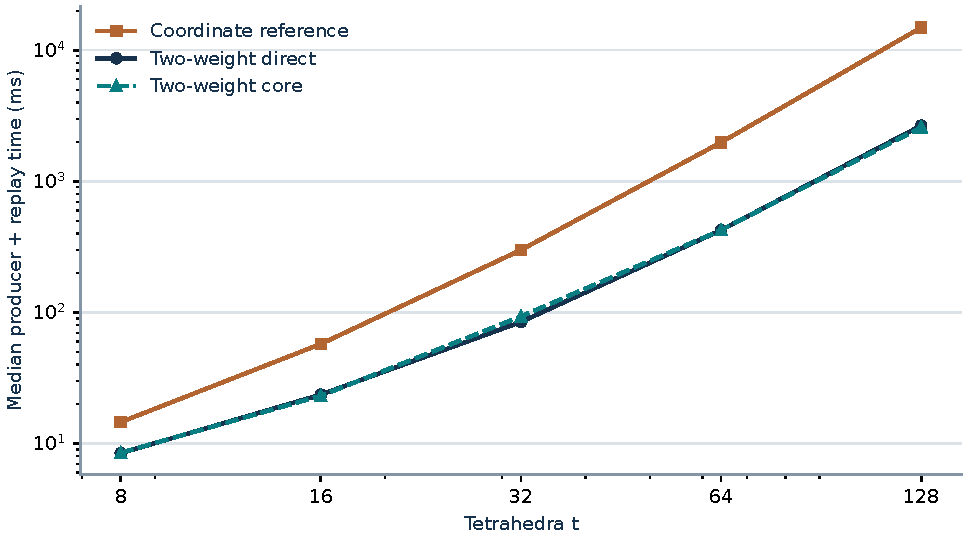
\includegraphics[width=\linewidth]{figures/dimension_timing.pdf}
\caption{Observed dimension-family timings, on logarithmic axes. Connecting
segments guide the eye; they are not fitted asymptotic laws. Core and direct
curves nearly coincide because these vectors have no large removable content.}
\label{fig:dimension}
\end{figure}

At $t=128$, the direct and coordinate-reference medians are approximately
2.662 and 14.913 seconds. The paired reference/direct factor is 5.733.
The corresponding serialized certificates contain 3,579,367 and 6,082,406
bytes. Thus this family shows increasing practical benefit from the smaller
observer, including a particularly large reduction in coordinate-reference
verification work. It does not identify a universal exponent in $t$.

\begin{table}[H]
\centering\small
\begin{tabular}{rrrrrr}
\toprule
Exponent $b$ & Input $B$ & Reference (ms) & Direct (ms) & Core (ms) & Direct/core\\
\midrule
128 & 139 & 126.738 & 52.977 & 22.972 & 2.322$\times$\\
4,096 & 4,107 & 161.687 & 90.527 & 24.942 & 3.631$\times$\\
16,384 & 16,395 & 212.546 & 193.630 & 27.738 & 6.994$\times$\\
32,768 & 32,779 & 299.004 & 331.892 & 32.055 & 10.368$\times$\\
\bottomrule
\end{tabular}
\caption{Fixed $16$-tetrahedron core with $g=2^b$ and
$x_g=gD+(g+1)L$. All full-coordinate gcds are one.}
\label{tab:multiplicity}
\end{table}

\begin{figure}[H]
\centering
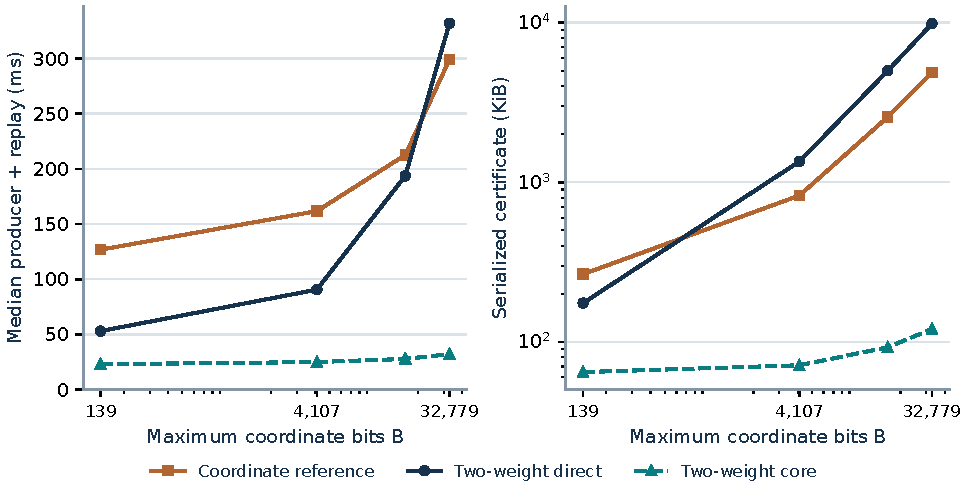
\includegraphics[width=\linewidth]{figures/multiplicity_timing_and_proofs.pdf}
\caption{The fixed-core family: observed time and certificate size.
Only the orbit-query core becomes small; original source coordinates,
divisor and restored binary multiplicities still appear in the computation.}
\label{fig:multiplicity}
\end{figure}

For the largest fixed-core input, with $B=32,779$, the direct and core
medians are 331.892 and 32.055 milliseconds; the paired improvement is
10.368. The certificates shrink from 10,081,806 to 123,278 bytes, a factor
of about 81.78. The reduced proof therefore remains dependent on $B$, as
predicted, but avoids repeating large multiplicities throughout the orbit
trace. Serialized size is not peak resident memory: the latter was not
measured.

\begin{table}[H]
\centering\small
\begin{tabular}{lrrrr}
\toprule
Family & Reference (ms) & Direct (ms) & Core (ms) & Direct/core\\
\midrule
M\"obius, even & 2.857 & 3.021 & 0.881 & 3.513$\times$\\
M\"obius, odd & 3.354 & 3.098 & 0.889 & 3.458$\times$\\
Klein, odd & 8.320 & 7.678 & 1.553 & 4.672$\times$\\
M\"obius + sphere/disc links & 13.149 & 10.391 & 2.089 & 4.973$\times$\\
\bottomrule
\end{tabular}
\caption{One-sided and mixed-link families at exponent 4,096. These include
parity restoration and the closed zero-signature collision.}
\label{tab:one-sided}
\end{table}

There are informative negative comparisons. On the $b=32,768$ meridian
mixture, the unreduced direct query is slower than the coordinate reference:
their median times are 331.892 versus 299.004 milliseconds, with a paired
reference/direct ratio of 0.900. The even M\"obius example similarly gives
a ratio of 0.945. The core mode is faster on both examples. On a primitive
$t=32$ meridian, reduction increases the median from 84.474 to 93.117
milliseconds; the paired direct/core ratio is 0.912. These measurements
support an explicit choice of representation, not a universal replacement
claim.

Across all cases, the paired A/A ratios range from 0.915 to 1.028. Five repeats are adequate for a transparent exploratory comparison, but do not establish statistical significance for small differences. No confidence interval, runtime-exponent fit, whole-knot speedup, or extrapolation to untested hard diagrams is claimed. The complete per-phase times, orders, exact inputs and proof hashes are in the raw JSON; the accompanying CSV exposes every reported median.

